\documentclass[UTF8]{ctexart}
\usepackage[left=2cm,right=2cm,top=2cm]{geometry}
\usepackage{amsmath}
\usepackage{enumitem}
\usepackage{float}
\usepackage{threeparttable}
\usepackage{caption}
\usepackage{multirow}
\usepackage{graphicx}
\usepackage{listings}
\usepackage{color}
\definecolor{dkgreen}{rgb}{0,0.6,0}
\definecolor{gray}{rgb}{0.5,0.5,0.5}
\definecolor{mauve}{rgb}{0.58,0,0.82}
\lstset{frame=tb,
  language=C++,
  aboveskip=3mm,
  belowskip=3mm,
  showstringspaces=false,
  columns=flexible,
  basicstyle={\small\ttfamily},
  numbers=left,%设置行号位置none不显示行号
  %numberstyle=\tiny\courier, %设置行号大小
  numberstyle=\tiny\color{gray},
  keywordstyle=\color{blue},
  commentstyle=\color{dkgreen},
  stringstyle=\color{mauve},
  breaklines=true,
  breakatwhitespace=true,
  escapeinside=`,%逃逸字符(1左面的键),用于显示中文例如在代码中`中文...`
  tabsize=4,
  extendedchars=false %解决代码跨页时,章节标题,页眉等汉字不显示的问题
}

\setlength\lineskiplimit{5.25bp}
\setlength\lineskip{5.25bp}

\title{计算方法第四次编程作业报告}
\author{崔士强 PB22151743}
\date{\today}

\bibliographystyle{plain}

\begin{document}

\maketitle

\section{问题描述}
实验的目的是实现Jacobi方法求解对称矩阵的特征值,并应用该方法于主成分分析(PCA)和矩阵的奇异值分解(SVD)。具体应用包括:
\begin{itemize}
    \item 使用PCA对数据进行有效压缩。
    \item 使用SVD对矩阵进行分解。
\end{itemize}

\section{问题分析}
\subsection{PCA主成分分析}
主要步骤包括:
\begin{enumerate}
    \item 数据去中心化并构造协方差矩阵 $\frac{1}{m}XX^T$。
    \item 应用Jacobi方法求解协方差矩阵的所有特征值。
    \item 选择最大的两个特征值对应的特征向量,构成视觉平面的基。
    \item 对数据进行投影,并可视化结果。
\end{enumerate}

\subsection{SVD分解}
主要步骤包括:
\begin{enumerate}
    \item 对矩阵 $A$ 应用Jacobi方法计算 $AA^T$ 和 $A^TA$ 的特征值。
    \item 分别计算 $AA^T$ 和 $A^TA$ 的特征向量,构成矩阵 $U$ 和 $V$。
    \item 构造对角阵 $\Sigma$,其中对角元素为特征值的平方根。
    \item 进行矩阵分解 $A = U\Sigma V^T$。
\end{enumerate}

\section{实验结果}
\subsection{结果展示}
程序的计算结果如下图所示
\begin{figure}[H]
  \centering
  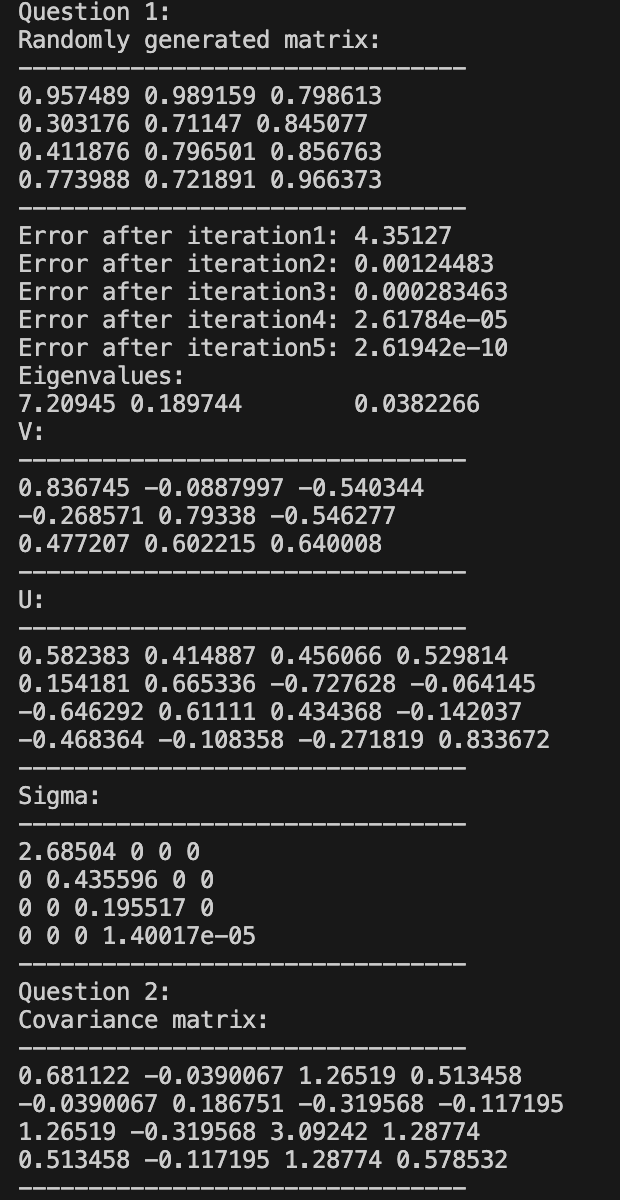
\includegraphics[scale=0.4]{program.png}
  \caption{计算结果}
\end{figure}
\begin{figure}[H]
  \centering
  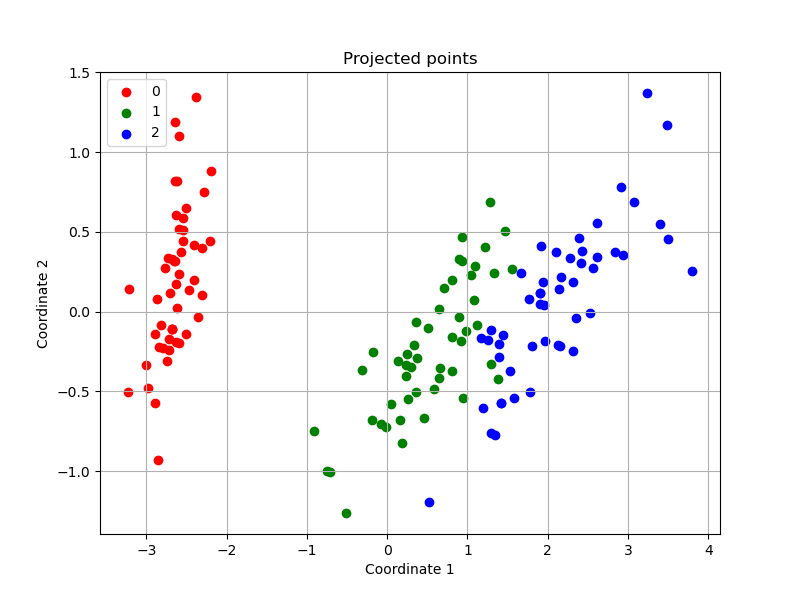
\includegraphics[scale=0.5]{result.png}
  \caption{可视化}
\end{figure}
\subsection{结果分析}
\begin{enumerate}
  \item 可以看到,Jacobi方法迭代中矩阵非对角元素平方和迅速下降
  \item 经计算验证,所求特征值是矩阵特征值的近似值
  \item 在可视化结果中,三个标签经降维后得到的点近似分布在三条直线附近
\end{enumerate}


\bibliography{math}

\end{document}
\iffalse
\begin{figure}[h]
    \centering
    \includegraphics[scale=0.5]{name.png}
    \caption{name}
\end{figure}
\fi
